\subsection{Vision Transformer (ViT)}
\label{appendix:vision_transformer}

The Vision Transformer (ViT) \cite{vision_transformer} by Google uses transformers for image classification, leveraging the encoder portion of the transformer architecture. While not a video synthesis model, its foundational principles influence many T2V models.

Traditional CNNs extract local spatial features but struggle with long-range dependencies. ViT addresses this by using transformers' attention mechanism, capturing global dependencies. It consists of patch embeddings, positional embeddings and a transformer's encoder.

In their paper, they found that ViT scale more effectively for visual recognition than traditional CNN networks.

\begin{figure}
    \centering
    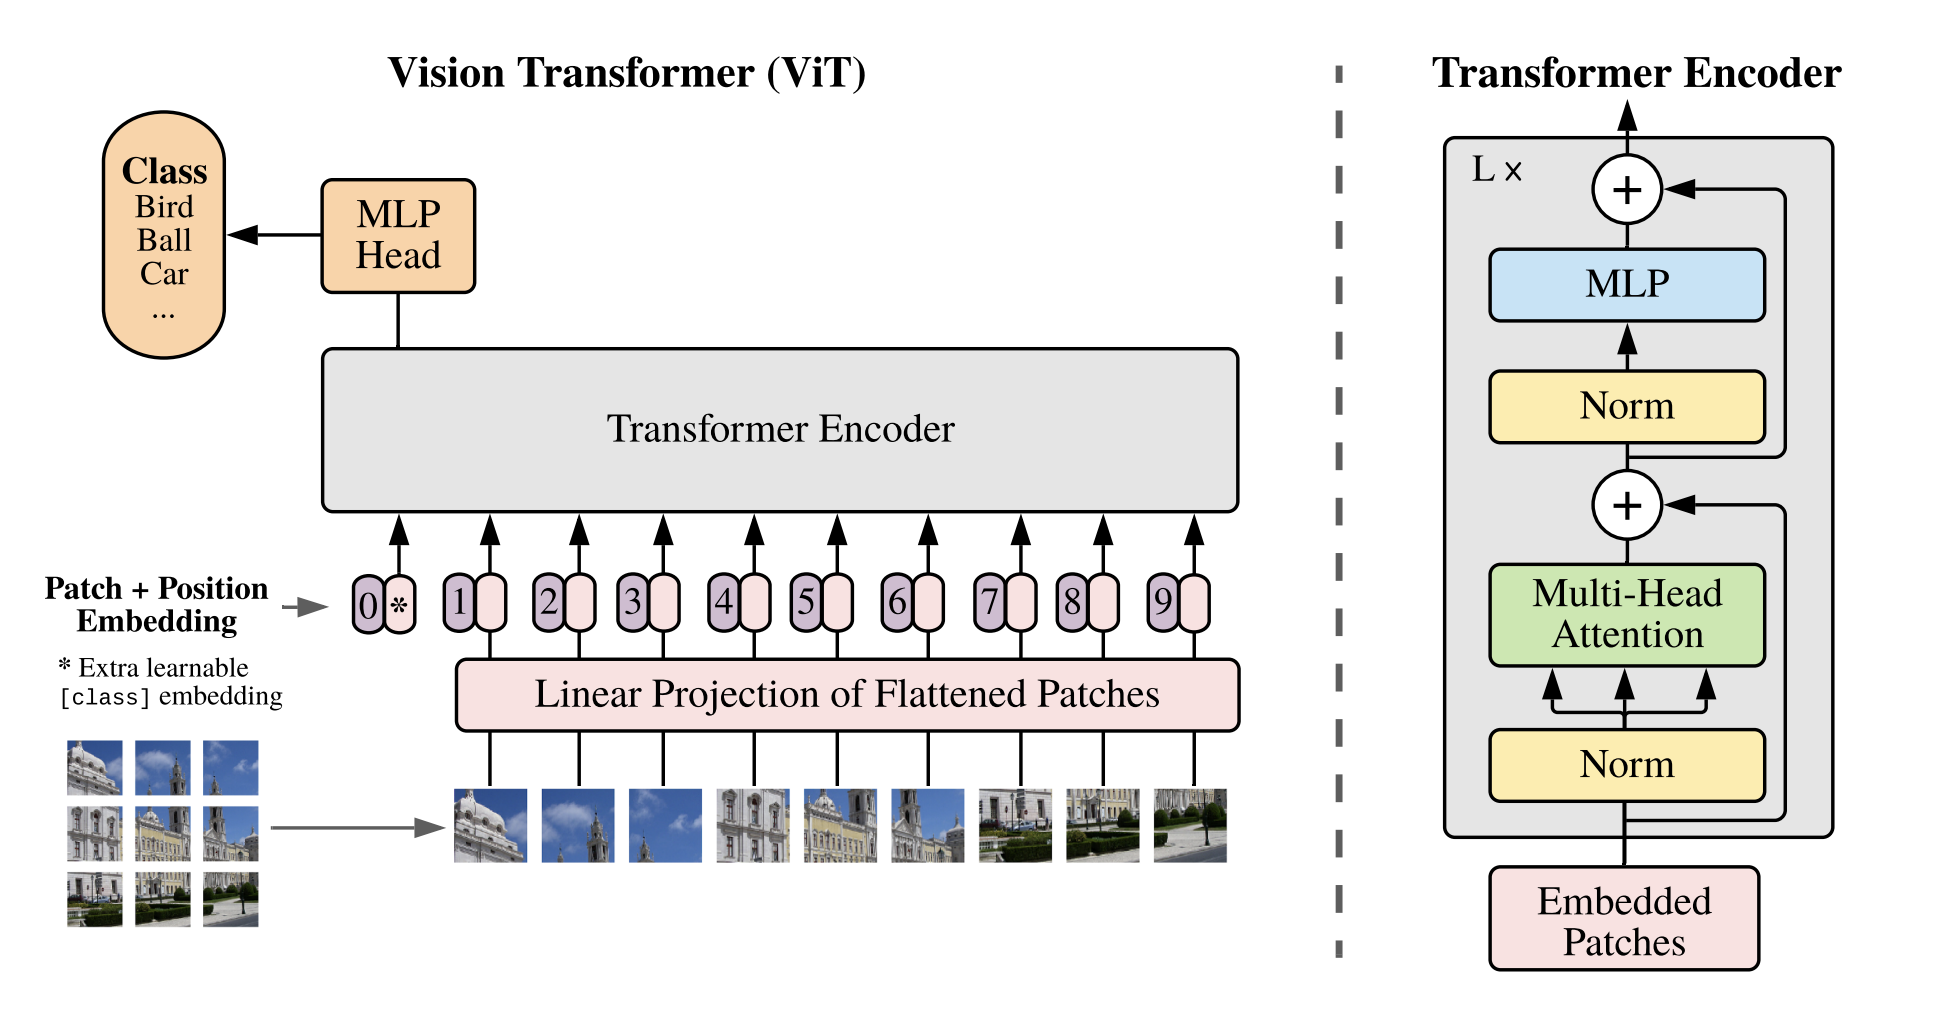
\includegraphics[width=0.6\textwidth]{images/appendix/vision_transformer/architecture.png}
    \caption{Vision Transformer (ViT) architecture \cite{vision_transformer}. The first patch + position embedding is the CLS token (classification token) which is used for image classification (its value is changed when the model learns to classify images) \cite{vision_transformer}.}
\end{figure}

\textbf{Patch embeddings}: The input image is divided into non-overlapping patches (e.g., $16\times 16\times 3$), flattened into vectors, and linearly projected into fixed-size vectors ($D$):

\[ \text{Projected} = \text{FlattenPatch} \times W + b \]

\textbf{Position embeddings}: Each patch is assigned a spatial position encoded using sinusoidal embeddings (section \ref{subsec:sinusoidal_embeddings}).

\textbf{Combining the embeddings}: The patch embeddings and the positional embeddings are summed together element-wise (\textbf{and not concatenated}, channel-wise) to form the input to the encoder.

\textbf{Transformer encoder}: The patch embeddings and positional embeddings are fed to the transformer encoder. It uses self-attention to weight the importance of each patch embedding in order to capture long-range relationships between patches.

\textbf{Classification head}: An MLP layer is used to classify the image based on the encoder's output.

ViT effectively models relationships across image patches, offering a scalable alternative to CNNs. Its success has influenced the use of transformers in image and video synthesis.